\documentclass[french]{beamer}
\usepackage{graphicx}
\usepackage{caption}

\usepackage[utf8]{inputenc}
\usepackage[T1]{fontenc}
\usepackage{lmodern}
\usepackage{amsmath, amssymb}
\usepackage{bbm}
\usepackage{algorithm}
\usepackage{algpseudocode}
\usepackage{babel}


%CHOIX DU THEME et/ou DE SA COULEUR
% => essayer différents thèmes (en décommantant une des trois lignes suivantes)
%\usetheme{PaloAlto}
%\usetheme{Madrid}
%\usetheme{Copenhagen}
%\usetheme{CambridgeUS}

\usetheme{Hannover}

\useoutertheme[height=0pt,left]{sidebar}
\usecolortheme{beaver}
\setbeamercolor*{titlelike}{parent=structure}
\useinnertheme{circles}
\setbeamertemplate{frametitle}[default][right]



% => il est possible, pour un thème donné, de modifier seulement la couleur
%\usecolortheme{crane}
%\usecolortheme{seahorse}

%\useoutertheme[left]{sidebar}


%Pour le TITLEPAGE
\title{Analyse en Ondelettes}
\subtitle{Projet mathématiques-informatique}
\author[Rouyer, Gervais, Boulahia ]{ Chloé Rouyer, Pierre Gervais,  Souhaib Boulahia}
\date{\today}
\institute{Université Paris Diderot}


\begin{document}

\begin{frame}
	\titlepage
\end{frame}


\begin{frame}{Introduction}
	
	\begin{figure}[h]
		\centering
		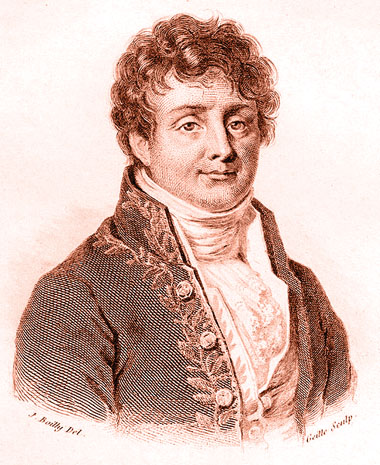
\includegraphics[width=100pt]{Fourier.jpg}
		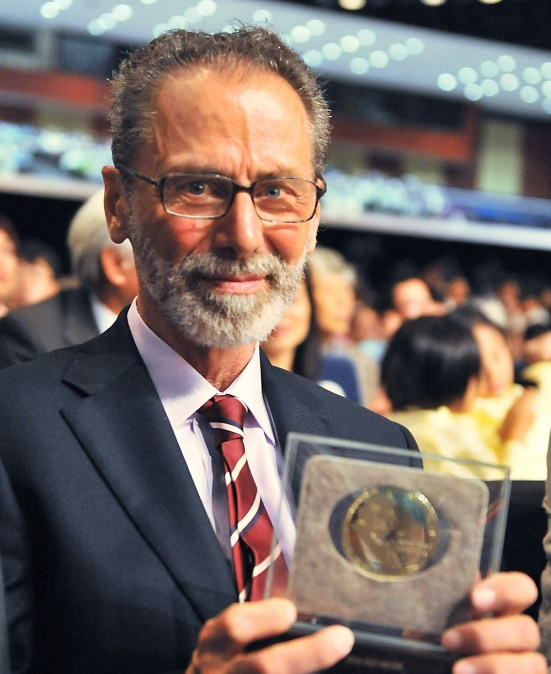
\includegraphics[width=100pt]{Meyer.jpg}
		\caption*{Joseph Fourier (1768 -1830) et Yves Meyer (1939- )}
	\end{figure}
	
\end{frame}

\begin{frame}{Sommaire}
	\tableofcontents
\end{frame}

\section{Outils}

\subsection{Analyse de Hilbert}
\begin{frame}{Problématique}
	
	\begin{itemize}
		\item<1-> Signaux : fonctions $\mathbb{R}^n \rightarrow \mathbb{R}^m$
		\item<2-> On veut généraliser les outils de la géométrie euclidienne
	\end{itemize}
		
\end{frame}

\begin{frame}{Problématique}
	\begin{itemize}
		\item<1-> $\ell^2$ et la famille $\{x_n = \delta(n - \cdot)\}_n$
		\item<2-> But : pouvoir écrire $$u = \sum_{n = 0}^{\infty} u_n x_n$$
	\end{itemize}
\end{frame}

\begin{frame}{Espace de Hilbert}
	Un \textit{espace de Hilbert} est la donnée
	\pause
	\begin{itemize}
		\item D'un espace vectoriel réel $E$ \pause
		\item D'un produit scalaire $\langle \cdot, \cdot \rangle$ défini sur $E$ \pause
		\item tel que $E$ soit complet pour la norme induite par ce produit scalaire
	\end{itemize}
\end{frame}

\begin{frame}{Exemple d'espace hilbertien}
	$\ell^2$ avec le produit scalaire défini par $\displaystyle \langle u, v \rangle = \sum_{n = 0}^{\infty} u_n \overline{v_n}$
\end{frame}

\begin{frame}{Espace de Hilbert séparable}
	$E$ est dit \textit{séparable} s'il existe $\mathbf{g} = \{g_n\}_{n \in \mathbb{N}}$ tel que $\overline{\mathbf{g}} = E$.
\end{frame}

\begin{frame}{Séparabilité et base hilbertienne}
	$E$ est séparable si et seulement s'il admet une base hilbertienne
	\pause
	où une \textit{base hilbertienne} est une famille orthonormée \textbf{totale}, c'est-à-dire une famille orthonormée $\mathcal{B}$ telle que $\text{Vect}(\mathcal{B})$ soit dense dans $E$.
\end{frame}

\begin{frame}{$E$ (de dimension infinie) séparable $\Longleftrightarrow$ $E$ admet une base hilbertienne}
	$\mathbf{g} = \{g_n\}_{n \in \mathbb{N}} \subset E$ telle que $\overline{\mathbf{g}} = E$.\\
	\pause
	On construit par récurrence $\mathbf{f} = \{f_n\}_{n \in \mathbb{N}}$ de manière à ce que $\{f_0, \cdots f_n\}$ soit orthonormale pour tout $n$. \\
	\pause
	
	On pose $f_0 = \frac{g_0}{\|g_0\|}, ~ g_0 \neq 0$.
	
	\pause
	On construit par récurrence $f_{n+1}$ à l'aide de $f_0, \cdots f_n$ :
	\pause
	\begin{itemize}
		\item on choisit $x \in \text{Vect} (g_0 \cdots g_m)  \setminus \text{Vect} (f_0 \cdots f_n)$, avec $m$ le plus petit possible pour que $x$ existe \pause (il existe car $E$ est de dimension infinie). \pause Ainsi $\text{Vect} (g_0 \cdots g_m) = \text{Vect} (f_0 \cdots f_n, x)$
		\pause
		\item on orthogonalise la nouvelle famille : $\displaystyle y = x - \sum_{k = 0}^{n} \langle y, f_k \rangle f_k$
		\pause
		\item on normalise le nouveau vecteur : $f_{n+1} = \frac{y}{\|y\|}$
	\end{itemize}
	
	\pause
	En passant à l'adhérence : $E = \overline{\mathbf{g}} \subset \overline{\text{Vect}(\mathbf{f})} \subset E$
\end{frame}

\subsection{Espaces de Lebesgue}

\begin{frame}{Espaces de Lebesgue}
	Soit $(X, \mathcal{A}, \mu)$ un espace mesuré.\\
	\pause
	$$\mathcal{L}^p(X) = \left\{f ~: ~ X \to \mathbb{C} \text{ mesurable} ~ | ~ \int_X |f|^p d\mu < \infty \right\}$$
	\pause
	$$\|f\|_p = \left(\displaystyle \int_X |f|^p d\mu \right)^{\frac{1}{p}}$$
\end{frame}

\begin{frame}{Espaces de Lebesgue}
		Soit la relation d'équivalence définie par $f \mathcal{R} g \Longleftrightarrow f \equiv g$ p.p.
		\pause
		$$L^p(X) = \mathcal{L}^p(X)/\mathcal{R}$$
		\pause
		$(L^p(X), \|\cdot\|_p)$ est alors normé ... \pause et complet !
\end{frame}


\section{Première approche : Analyse de Fourier}
\subsection{Série de Fourier}
\begin{frame}{Séries de Fourier}
	La décomposition en série de Fourier s'applique aux fonctions périodiques.\\ 
	
	Dans $L^2(\mathbb{T})$ : 
	\begin{itemize}
		\item<1-> Les $\{e^{-ikt}\}_{k \in \mathbb{Z} }$ forment une base Hilbertienne
		
		\item<2-> Toute fonction de $L^2(\mathbb{T})$ se décompose dans la base des $\{e^{-ikt}\}_{k \in \mathbb{Z}}$
		
		\item<3-> On définit les coefficients de Fourier par\\ $c_k =  \langle f,e^{-ikt} \rangle = \frac{1}{2\pi} \int_{0}^{2\pi} f(t) \overline{e^{-ikt}}dt $ 
		
		\item<4-> Et 
		$	S_N(f) = \sum_{k = -N}^N c_k(f) e^{-ikt} $
		
		\item<5-> Avec $ \lim\limits_{N \to \infty} \| S_N(f) - f \|_2  = 0 $ 
		
	\end{itemize}
	
\end{frame}

\begin{frame}{Preuve de $ \lim\limits_{N \to \infty} \| S_N(f) - f \|_2  = 0$ }
	
	Soit $f \in L^2(\mathbb{T})$, soit $\varepsilon > 0$.\\
	Soit $f_0 \in L^2(\mathbb{T})$ une fonction continue telle que 
	$ | f_0 - f | < \varepsilon $\\
	\pause
	Soit $F_0$ tel que $f_0(t) = F_0(e^{it})$\\ 
	Il existe un polynôme trigonométrique $P$ tel que pour tout t, $\|f_0(t) - P(t)\| < \varepsilon$\\
	Ce qui permet de déduire que: \\
	\pause
	\begin{align*}
	\| S_N(f) -f \|_2 &\leqslant \|S_N(f) - S_N(P)\|_2 + \| S_N(P) - P \|_2 + \| f- P \|_2 \\
	&	\leqslant 2 \| f - P\|_2 + \| S_N(P) - P\|_2 \ \\
	& \leqslant 2 \| f - P\|_2  \\
	& \leqslant 2 \| f - f_0\|_2 + 2 \| f_0- P\|_2 \\
	& \leqslant 4 \varepsilon
	\end{align*}
	
	
\end{frame}



\begin{frame}{Séries de Fourier}	
	Vitesse de décroissance des coefficients. \\
	
	Si $f \in \mathcal{C}^k$ alors : \\
	$$ | c_p(f) | \leqslant \frac{C}{|p|^k} $$
	
	
\end{frame}


\subsection{Transformée de Fourier}
\begin{frame}{Transformée de Fourier}
	
	Transformée de Fourier pour $f \in  L^1(\mathbb{R})$
	$$ \mathcal{F}[f](\xi) = F(\xi)= \int_{-\infty}^{+\infty}f(t)e^{-i\xi t}dt $$ 
	
	\pause
	Transformée de Fourier inverse pour $f, F \in  L^1(\mathbb{R})$ et $f$ continue
	$$ \overline{\mathcal{F}}[F](t) = f(t)=\frac{1}{{2\pi}} \int_{-\infty}^{+\infty}F(\xi)e^{i \xi t}dt $$
	
\end{frame}


\begin{frame}
	\begin{figure}[h]
		\centering
		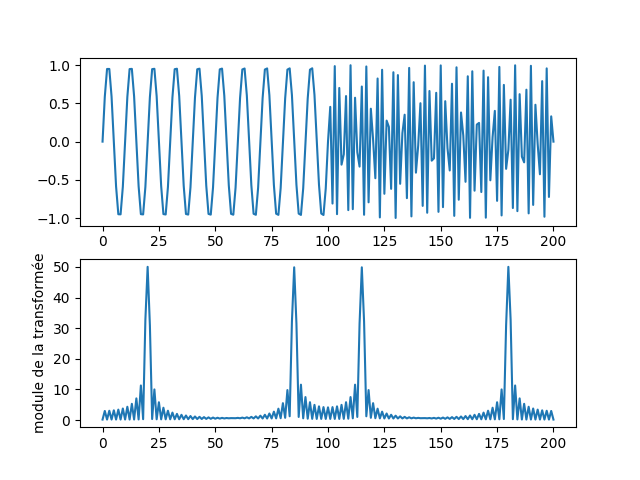
\includegraphics[width=150pt]{successifs.png}
		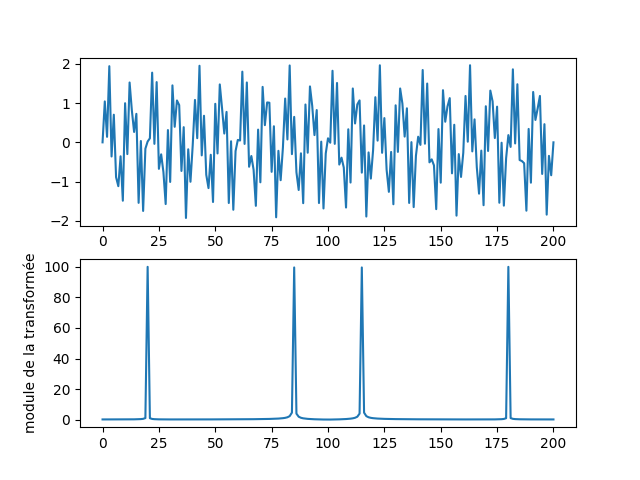
\includegraphics[width=150pt]{simultanes.png}
		\caption*{2 signaux ayant des transformées de Fourier similaires}
		
		\pause	
		
		$$ F(\xi, \tau)= \int_{-\infty}^{+\infty}f(t)e^{-i \xi t} \overline{w(t - \tau)}dt$$
	\end{figure}
	
\end{frame}






\section{Ondelettes et application}

\subsection{Analyse multi-résolution}

\begin{frame}{Analyse multi-résolution}
	
	\begin{figure}[h]
		\centering
		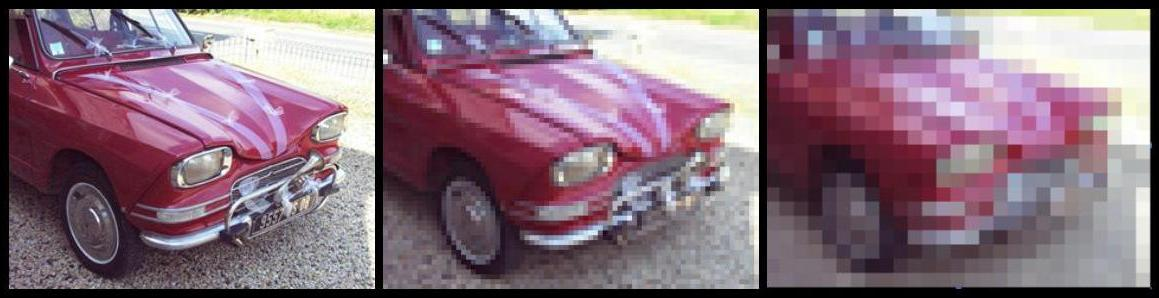
\includegraphics[width=250pt]{Pierre/Resolution_wikipedia.jpg}
		\caption*{Une image de voiture pour trois résolutions différentes}
	\end{figure}
\end{frame}

\begin{frame}{Analyse multi-résolution}
	Une \textit{analyse multi-résolution} de $L^2(\mathbb{R})$ est une famille de sous-espaces fermés $\{V_n\}_{n \in \mathbb{Z}} \subset L^2(\mathbb{R})$ telle que
	
	\pause
	$$\forall n \in \mathbb{Z}, ~ V_{n} \subset V_{n+1}$$

	\pause
	$$\forall n \in \mathbb{Z}, \forall f \in L^2(\mathbb{R}), ~ f \in V_n \Longleftrightarrow f (2 \, \cdot ) \in V_{n+1}$$
	
	\pause
	Il existe $\varphi$ telle que $\{\varphi_k = \varphi(\, \cdot + k)\}_{k \in \mathbb{Z}}$ forme une base orthonormée de $V_0$

	\pause
	$$\overline{\bigcup V} = L^2(\mathbb{R})$$
	
	\pause
	$$\bigcap V = \{0\}$$

	\pause			
	$\varphi$ est appelée \textit{fonction d'échelle}.
\end{frame}


\begin{frame}{L'espace de détails}
	L'espace $V_{n+1}$ est plus "fin" que $V_n$.\\
	\pause
	Soit $P_n ~ : ~ V_{n+1} \rightarrow V_n$ la projection orthogonale \pause $$W_n = \ker (P_n) \pause = V_{n+1} \cap V_n^\bot$$
	\pause
	On définit l'\textit{espace de détails} par
	$$V_{n+1} = W_n \oplus V_n$$\\
\end{frame}

\begin{frame}{L'espace de détails}
	\begin{align*}
		\onslide<1->{V_n &= V_{n-1} \oplus W_{n-1} \\}
		\onslide<2->{&= V_{n-2} \oplus W_{n-2} \oplus W_{n-1} \\}
		\onslide<3->{&= V_{n-3} \oplus W_{n-3} \oplus W_{n-2} \oplus W_{n-1} \\}
		\onslide<4->{ & \vdots \\ &= \underbrace{\bigcap V}_{\{0\}} \oplus \left(\bigoplus_{k < n} W_k\right) \\}
	\end{align*}

	\onslide<5->{Et en faisant l'union pour tout $n \in \mathbb{Z}$ à droite et à gauche
		$$\bigcup_{n \in \mathbb{Z}} V_n = \bigoplus_{n \in \mathbb{Z}} W_n \onslide<6-> = V_0 \oplus \left(\bigoplus_{n \in \mathbb{N}} W_n\right)$$
	}
\end{frame}

\begin{frame}{Les ondelettes}
	$\{W_n\}_{n \in \mathbb{Z}}$ n'est pas une suite croissante mais on conserve l'auto-similarité.
	\pause
	$$f \in W_0 \Longleftrightarrow f(2 \cdot ) \in W_1 \Longleftrightarrow f(2^n \cdot) \in W_n$$
	
	\pause
	Il existe $\psi \in W_0$ tel que \\
	\pause
	\begin{itemize}
		\item $\{\psi(\cdot + k)\}_{k \in \mathbb{Z}}$ est une base orthonormée de $W_0$
		\pause
		\item $\displaystyle \int_{\mathbb{R}} \psi(t) dt = 0$ \\
	\end{itemize}
	
	\pause
	$\{\sqrt{2^n} \psi(2^n\cdot - k)\}_{k \in \mathbb{Z}}$ est une base orthonormée de $W_n$.\\
	
	\pause	
	
	La famille définie par $\psi_{n, k}(t) = \sqrt{2^n}(2^n t - k)$ forme une famille orthonormée de $\displaystyle \bigoplus_{n \in \mathbb{Z}} W_n$\\
	\pause
	$\{\psi_{n, k}\}_{n, k \in \mathbb{Z}}$ est une base hilbertienne de $L^2(\mathbb{R})$ !
\end{frame}

\begin{frame}
	De $\displaystyle \bigcup_{n \in \mathbb{Z}} V_n = \bigoplus_{n \in \mathbb{Z}} W_n = V_0 \oplus \left(\bigoplus_{n \in \mathbb{N}} W_n\right)$

	\pause

	on déduit pour tout $f \in L^2(\mathbb{R})$
	
	$$f= \sum_{\substack{k \in \mathbb{Z} \\ n \in \mathbb{Z}}} \langle \psi_{n, k}, f \rangle \psi_{n, k} = \sum_{k \in \mathbb{Z}} \langle \varphi_k, f \rangle \varphi_k + \sum_{\substack{k \in \mathbb{Z} \\ n \in \mathbb{N}}} \langle \psi_{n, k}, f \rangle \psi_{n, k} $$
\end{frame}

\begin{frame}{Ondelette de Haar}
	L'ondelette de Haar est définie par :
	$$ \psi(t) = \begin{cases}
	-1&\text{si $0\leqslant t < \frac12$} \\
	1&\text{si $\frac12\leqslant t < 1$} \\
	0&\text{sinon} \\
	\end{cases}$$
	La fonction d'échelle associée est la fonction porte :
	$$ \varphi(t) = \begin{cases}
	1&\text{si $0\leqslant t < 1$} \\
	0&\text{sinon} \\
	\end{cases}$$
	Peu régulière, discontinue
\end{frame}

\begin{frame}{Ondelette chapeau mexicain}
	L'ondelette chapeau mexicain est définie par :
	$$ \psi(t) = \lambda \left(1-t^2\right) e^{-\frac{t^2}{2}} $$
	avec :
	$$\lambda = \frac{2}{\sqrt{2}\pi^{\frac14}}$$
\end{frame}

\begin{frame}{Algorithme d'encodage}
	On rappelle :
	$$\bigcup_{n \in \mathbb{Z}} V_n = V_0 \stackrel{\perp}{\oplus} \left(\bigoplus^{\bot}_{n \in \mathbb{N}} W_n\right)$$
	
	On peut décomposer tout fonction $f \in L^2(\mathbb{R})$ ainsi : $$f = \sum_{k \in \mathbb{Z}} \langle f,\varphi_k \rangle \varphi_k + \sum_{\substack{k \in \mathbb{Z} \\ n \in \mathbb{N}}} \langle f,\psi_{n, k} \rangle \psi_{n, k}$$
\end{frame}

\begin{frame}{Algorithme d'encodage}
	On manipule des fonctions $f \in L^2(\mathbb{R})$ de la forme $$f = \sum_{j = 0}^{2^{N_0} - 1} a_j \mathbb{1}_{[2^{-N_0}j, 2^{-N_0}(j+1)[}$$
	
	\begin{align*}
	\langle f, \psi_{n, k} \rangle &= \int_0^1 f(t) \overline{\psi_{n, k}(t)} dt \\&= \sum_{j=0}^{N-1} a_j \left(\Phi\left(\frac{j+1}N - \frac{k}{N}\right) - \Phi\left(\frac{j}N - \frac{k}{N}\right)\right)
	\end{align*}
	
	où $\Psi$ est une primitive de $\overline{\psi}$, $\Phi$ est une primitive de $\overline{\phi}$ et $N = 2^{N_0}$.
\end{frame}

\begin{frame}{Algorithme d'encodage}
	\begin{figure}[h]
		\centering
		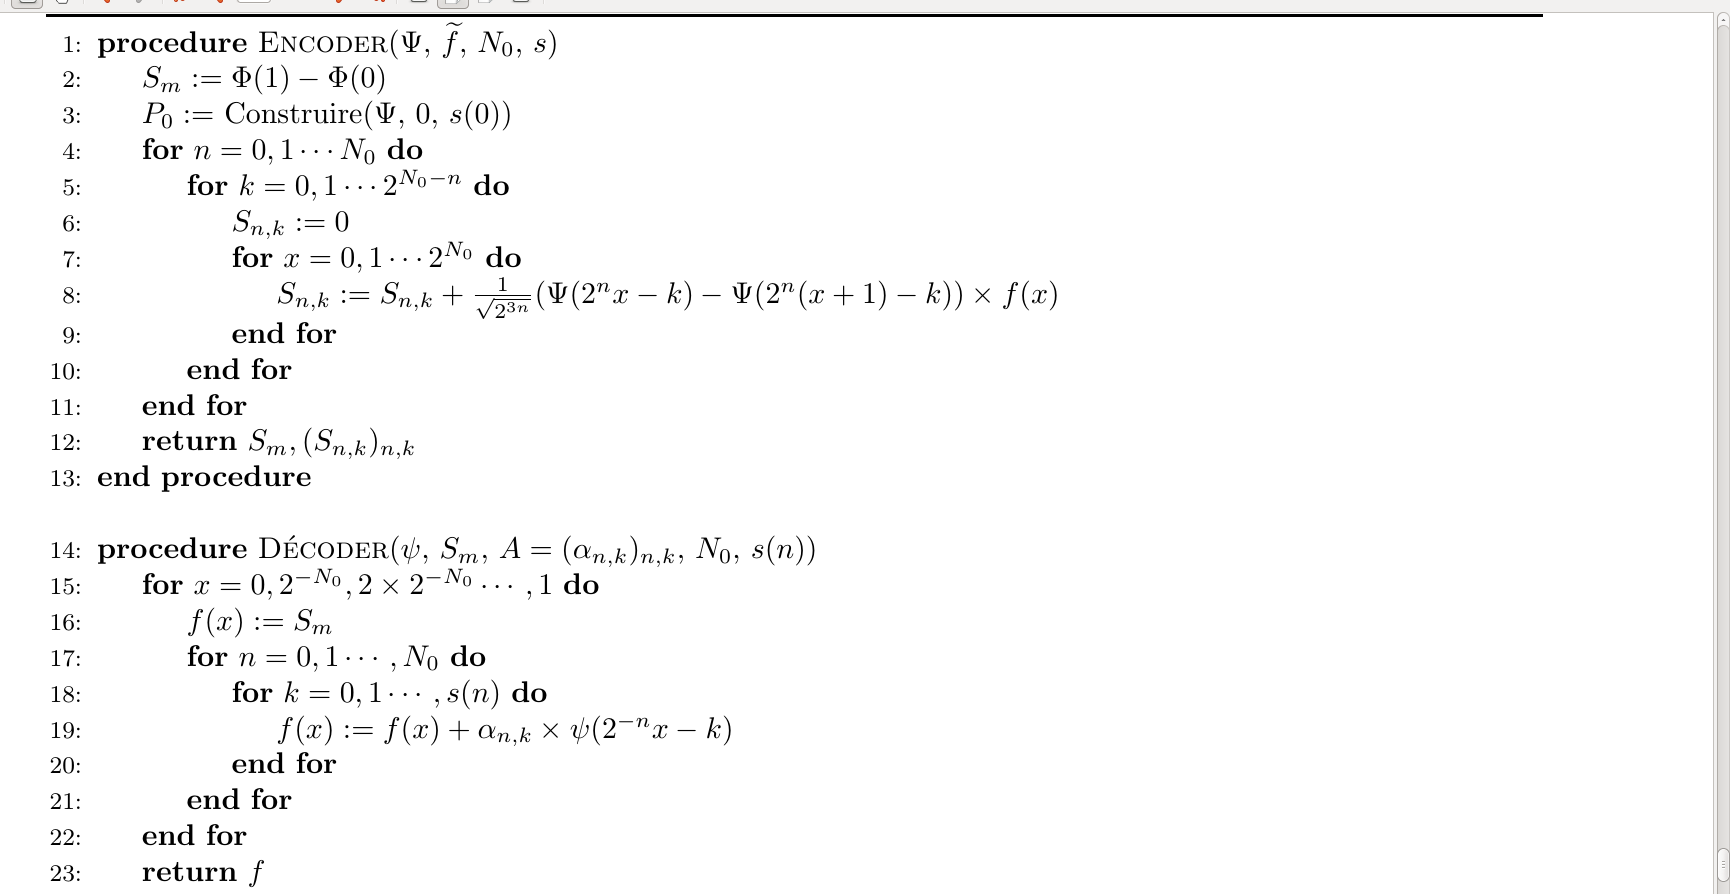
\includegraphics[width=300pt]{algo.png}

	\end{figure}

\end{frame}






\end{document}
















